\documentclass[10pt]{article}

%%% Работа с русским языком
\usepackage{cmap}					% поиск в PDF
\usepackage{mathtext} 				% русские буквы в фомулах
\usepackage[T2A]{fontenc}			% кодировка
\usepackage[utf8]{inputenc}			% кодировка исходного текста
\usepackage[english,russian]{babel}	% локализация и переносы

%%% Дополнительная работа с математикой
\usepackage{amsmath,amsfonts,amssymb,amsthm,mathtools} % AMS
\usepackage{icomma} % "Умная" запятая: $0,2$ --- число, $0, 2$ --- перечисление

%% Номера формул
\mathtoolsset{showonlyrefs=true} % Показывать номера только у тех формул, на которые есть \eqref{} в тексте.

%% Шрифты
\usepackage{euscript}	 % Шрифт Евклид
\usepackage{mathrsfs} % Красивый матшрифт
\usepackage{fancyhdr}

%% Работа с гиперссылками
\usepackage{xcolor}
\usepackage{hyperref}
% Цвета для гиперссылок
\definecolor{linkcolor}{HTML}{799B03} % цвет ссылок
\definecolor{urlcolor}{HTML}{799B03} % цвет гиперссылок
\hypersetup{pdfstartview=FitH,  linkcolor=linkcolor,urlcolor=urlcolor, colorlinks=true}

%% Работа с картинками
\usepackage{graphicx}
\graphicspath{{pictures/}}
\DeclareGraphicsExtensions{.pdf,.png,.jpg,.eps}

%% Геометрия и отступы
\usepackage{geometry}
\geometry{verbose,a4paper,tmargin=2.0cm,bmargin=2.0cm,lmargin=1.0cm, rmargin=1.0cm}

%% Свои команды
\pagenumbering{arabic}

%%% Заголовок
\author{Кравцов Михаил Викторович}
\title{Выпускная квалификационная работа \textbf{<<Селективный экспресс-метод измерения времени продольной спиновой релаксации в твердотельных системах>>}}
%\date{\today}

\pagestyle{fancy}
\fancyhead{}
\fancyfoot{}
\fancyhead[R]{\textsc{ВКР Кравцов М.В. Москва 2022}}

\begin{document} % конец преамбулы, начало документа
	
\maketitle	
\newpage
\tableofcontents
\newpage

\twocolumn
\section{Измерение}\label{measurment}

Уравнение на эволюцию спина состоит из двух слагаемых: накачки и релаксации:

\begin{equation}\label{eq:DE}
\frac{dS}{dt} = P - \frac{S}{T}
\end{equation}

\begin{figure}[h]
	\includegraphics[scale = 0.4]{rf_on_off.png}
	\caption{Модуляция радиочастотного поля по времени}
	\label{fig:rf_on_off}
\end{figure}

На рис. \ref{fig:rf_on_off} видно, что половину периода синхронного детектирования рч-поле выключено и спины релаксируют со временем $T_1$, тогда как во второй половине периода в релаксацию вмешивается рч-поле, что меняет время релаксации на $T_1'$. \\

Таким образом, возбуждение спинов под действием рч-поля будет обладать следующей зависимостью:

\begin{figure}[h]
	\includegraphics[scale = 0.4]{excitation.png}
	\caption{Изменение проекции спина на ось, параллельную направлению магнитного поля, $\Delta S_{z}(t)$}
	\label{fig:excitation}
\end{figure}

\begin{equation}\label{eq:Soff}
S_{off} = PT_1 + (S_0 - PT_1)e^{-\frac{t}{T_1}}, \ t \in \left(  0, \frac{\pi}{\omega} \right) 
\end{equation}

\begin{equation}\label{eq:Son}
S_{on} = PT_1' + (S_0 - PT_1')e^{-\frac{t}{T_1'}}, \ t \in \left(  \frac{\pi}{\omega}, \frac{2\pi}{\omega} \right) 
\end{equation}

Измерение проводилось методикой синхронного детектирования, таким образом, для получения сигнала, нужно свернуть \eqref{eq:Soff}, \eqref{eq:Son} с $\cos{\omega t}$ и $\sin{\omega t}$, соответственно.

\footnotesize
\begin{eqnarray}\label{eq:ESRcos}
\\
Re(ESR) \simeq \omega\int_{0}^{\frac{\pi}{\omega}} e^{-\frac{t}{T_1}} \cos(\omega t)dt + \omega \int_{\frac{\pi}{\omega}}^{\frac{2 \pi}{\omega}} e^{-\frac{t}{T_1}} \cos(\omega t)dt = \\
= \frac{\omega T_1 \left( S_0 - PT_1 \right) \left( e^{-\frac{\pi}{\omega T_1}} + 1 \right) }{1 + T_1^2 \omega} + \frac{\omega T_1' \left( S_0 - PT_1' \right) \left( e^{-\frac{\pi}{\omega T_1'}} + e^{-\frac{2 \pi}{\omega T_1'}} \right) }{1 + T_1'^2 \omega}
\end{eqnarray}

\begin{eqnarray}\label{eq:ESRsin}
\\
Im(ESR) \simeq \omega\int_{0}^{\frac{\pi}{\omega}} e^{-\frac{t}{T_1}} \sin(\omega t)dt + \omega \int_{\frac{\pi}{\omega}}^{\frac{2 \pi}{\omega}} e^{-\frac{t}{T_1}} \sin(\omega t)dt = \\
= \frac{\omega^2 T_1^2 \left( S_0 - PT_1 \right)  \left( e^{-\frac{\pi}{\omega T_1}} + 1 \right) }{1 + T_1^2 \omega} + \frac{\omega^2 T_1'^2 \left( S_0 - PT_1' \right)  \left( e^{-\frac{\pi}{\omega T_1'}} + e^{-\frac{2 \pi}{\omega T_1'}} \right) }{1 + T_1'^2 \omega} 
\end{eqnarray}
\normalsize

При условии $\frac{1}{T_1} - \frac{1}{T_1'} << 1$:

\begin{equation}\label{eq:ESR}
ESR \approx \sqrt{\frac{1}{1 + \omega^2 T_1^2}}
\end{equation}

\begin{figure}[h!]
	\centering
	\includegraphics[scale = 0.55]{ESR.png}
	\caption{Резонанс в кристалле перовскита, детектируемый оптически с аппроксимацией согласно \eqref{eq:ESR}}
	\label{fig:resonance}
\end{figure}

\newpage

\section{Магнитное поле в образце}

\begin{figure}[h!]
	\centering
	\includegraphics[scale = 0.2]{magn_scheme.png}
	\caption{Геометрия сверхпроводящей проволоки, относительно образца. a - ширина соленоида, b - высота, s - расстояние от крайней точки соленоида до образца, l - диаметр трубки}
	\label{fig:mag_scheme}
\end{figure}

Соленоид представляет из себя витки сверхпроводящей проволоки диаметром $d$, огибающей трубку. 

\subsection{Вычисление поля в образце}

Рассмотрим 1 виток проволоки. Найдем поле на ее оси.

\begin{figure}[h!]
	\centering
	\includegraphics[scale = 0.1]{coil}
	\caption{Поле от витка}
	\label{fig:coil}
\end{figure}

По закону Био-Савара-Лапласа, модуль магнитной индукции $\vec{B}$:

\begin{equation}\label{eq:BSR}
B = \frac{\mu_0}{4 \pi}  \int_{0}^{2 \pi r_0}  \frac{I r_0^2}{r^3}\,dl  = \mu_0 \frac{I r_0^2}{2 r^3} = \mu_0 \frac{I}{2 r_0} \sin^3{\beta}
\end{equation}

Магнитное поле от кольцевого тока $I n dx$ витка соленоида с линейной плотностью витков $n$.

\begin{equation}\label{eq:dB}
dB = \mu_0 \frac{I n dx}{2 r_0} \sin^3{\beta} = \{x = r_0 \cot(\beta)\} = - \frac{I n \sin{\beta} d\beta}{2}
\end{equation}

После интегрирования имеем

\begin{equation}\label{eq:B}
B = \mu_0 \frac{I n}{2} (\cos(\beta_2) - \cos(\beta_1))
\end{equation}

где $\beta_2$ и $\beta_1$ - углы, под которым из точки образца видны крайние точки соленоида на рис. \ref{fig:mag_scheme}

Рассмотрим поле, создаваемое первым рядом обмоток:

\begin{equation}\label{eq:B1}
B_1 = \mu_0 \frac{I}{2 d} (\frac{s+a}{\sqrt{(s+a)^2 + \frac{l^2}{4}}} - \frac{s}{\sqrt{s^2 + \frac{l^2}{4}}})
\end{equation}

Рассмотрим произвольный $y$ ряд обмоток. Поле, создаваемое им:

\begin{equation}\label{eq:By}
B_y = \mu_0 \frac{I}{2 d} (\frac{s+a}{\sqrt{(s+a)^2 + (\frac{l}{2} + d*y)^2}} - \frac{s}{\sqrt{s^2 + (\frac{l}{2} + d*y)^2}})
\end{equation}

Суммируя все вклады, получим 

\begin{equation}\label{eq:Btot}
B_{tot} = \sum_{y = 0}^{N_b - 1} B_y
\end{equation}

Для характерных параметров: 
$I = 30\ A$ 
$a = 1\ cm$ 
$b = 0.2\ cm$ 
$d = 0.3\ mm$ 

Зависимость поля от расстояния до образца:

\begin{figure}[h!]
	\centering
	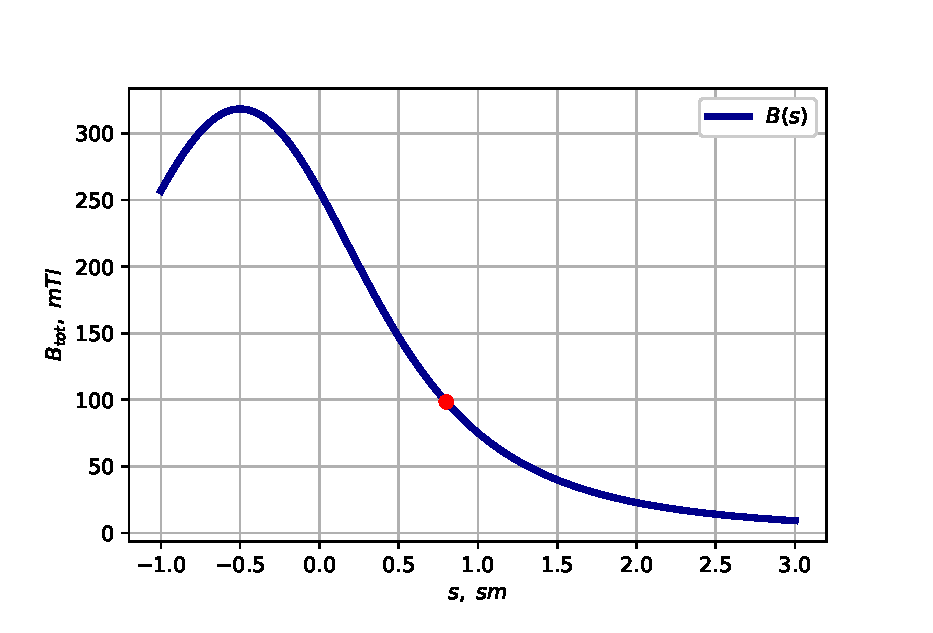
\includegraphics[scale = 0.45]{B_s}
	\caption{Зависимость поля в образце от его расстояния до соленоида}
	\label{fig:B_s}
\end{figure}

Для расстояния $s = 0.45\ cm$ \colorbox{yellow}{$B_{tot} \approx 157\ mTl$}

\subsection{Длина проволоки}

Посчитать число витков можно исходя из рис. \ref{fig:mag_scheme}. Число "строк" $N_a = \frac{a}{d} = \frac{1}{0.025} = 40$, число "столбцов" $N_b = \frac{b}{d} = \frac{0.2}{0.025} = 8$. \\

Таким образом, в соленоиде будет 320 витков со средним радиусом $<r> = \frac{l}{2} + \frac{b}{2} = 1.1\ cm$. То есть, длина проволоки $\colorbox{yellow}{L} = 2 \pi <r> N_{tot} \approx \colorbox{yellow}{22\ m}$

\section{Геометрия установки}\label{geometry}

\begin{figure}[h!]
	\centering
	\includegraphics[scale = 0.18]{ray_spread.png}
	\caption{\footnotesize Схема взаимного расположения образца, линзы и лучеделителя. s - расстояние от образца до выхода оптоволокна, d - расстояние от образца до линзы, f - расстояние от линзы до фотодиодов, t - расстояние от лучеделителя до фотодиодов, D - диаметр линзы. \normalsize}
	\label{fig:ray_spread}
\end{figure}

При желаемом размере пятна на образце в $d' = 1\ mm$ и угле аппертуры волокна $\alpha \approx 0.22\ rad \approx 12.7^{o} $ найдем $s = \frac{d'}{2}\ \frac{1}{\tan(\alpha)} \approx 4.5\ mm$

Оценим $d$ сверху, так как при сколь угодно большом d, пятно, приходящее на линзу будет превышать ее апертуру, вследствии чего будет собираться лишь часть света. Так как чистая апертура линз $\approx 0.9\ D$, запишем

\begin{equation}\label{eq:aperture}
(d + s)\tan(\alpha) = a = \frac{0.9D}{2}
\end{equation}

Условием на схождение луча после линзы является 

\begin{equation}\label{eq:ds}
d + s > F = \frac{f(d + s)}{f + d +s}
\end{equation}

Из \eqref{eq:aperture} и \eqref{eq:ds} следует, что $\frac{f(d + s)}{f + d +s} - s < d < 20.8\ mm$ \

Условие на $f$:\
при малом $f$ пятно на лучеделителе будет больше его апертуры, из-за чего будут потери в интенсивности.

Из подобия, найдем оценку на $f$ снизу:

\begin{equation}\label{eq:2a}
\frac{2a}{f} = \frac{0.9A}{L}
\end{equation}

Таким образом,

\begin{equation}\label{eq:f}
f > \frac{DL}{A}
\end{equation}

Из всех условий целесообразно использовать линзу с $F = 14.9\ mm, D \approx 12.7\ mm$ и лучеделитель с $L = 30\ mm$ и $A = 8\ mm$

Тогда при $d = 13.5\ mm, f = 90\ mm$ расстояние от линзы до лучеделителя составит $f - f_{min} \approx 42\ mm$, расстояние от лучеделителя до фотодиодов $t \approx 18\ mm$ 


\subsection{Прототип на 3D принтере}

\begin{figure}[h!]
	\centering
	\includegraphics[scale = 0.2]{assemble.png}
	\caption{Макет вставки, разработанный в среде 3D моделирования}
	\label{fig:assemble}
\end{figure}

Отдельные части компактного ОДМР-спектрометра напечатаны на 3D принтере так, чтобы вместе формировать готовую установку. В частности, было напечатано 6 составкных частей - бабина для сверхпроводящей проволоки, держатель оптоволокна, держатель образца с рч-катушкой, держателей фотодетекторов и держатель линзы с внешней нарезкой, позволяющей юстировать линзу вдоль направления распространения луча, варьируя параметр d из рис. \ref{fig:ray_spread}. 

\begin{figure}[h!]
	\centering
	\includegraphics[scale = 0.18]{wollaston.png}
	\caption{Призма Волластона. На вход приходит свет, поляризованный эллиптически, на выходе - 2 луча линейных перпендикулярных поляризаций.}
	\label{fig:wollaston}
\end{figure}

\newpage

\begin{thebibliography}{}
	
\end{thebibliography}

\end{document}